%\RequirePackage{atbegshi}
\documentclass{beamer}

\usetheme{default}
\usepackage{amssymb}
%\usepackage[cmex10]{amsmath}
\usepackage{stmaryrd}
\usepackage[english]{babel}
\usepackage{tikz,pgf,pgfplots}
\pgfplotsset{compat=newest}
\usepgflibrary{shapes}
\usepgfplotslibrary{polar}
\usetikzlibrary{%
  arrows,%
  mindmap,%mindmap
  calendar,%calendar
  decorations,%decorations
  snakes,%snakes
  shapes.misc,% wg. rounded rectangle
  shapes.arrows,%
	shapes.callouts, %
  shapes,%
  chains,%
  matrix,%
  positioning,% wg. " of "
  scopes,%
  decorations.pathmorphing,% /pgf/decoration/random steps | erste Graphik
	decorations.text, %
  shadows,%
  backgrounds,%
  fit,%
  petri%
}

% Radius of regular polygons
\newdimen\R
\R=0.8cm

\definecolor{tutorial}{RGB}{50,93,61}
\definecolor{forest}{RGB}{34,139,34}
\definecolor{tamu}{RGB}{80,0,0}


\title{Data Acquisition and Embedded Systems}
\author{Jean-Francois Chamberland\\
Gregory H. Huff}
\institute{Electrical and Computer Engineering}
\date{Texas A\&M University\\ August 31, 2015}

\setbeamertemplate{footline}[page number]
\setbeamertemplate{navigation symbols}{}
%\textcolor{black}{\insertframenumber / \inserttotalframenumber}}

\newlength\tikzheight
\newlength\tikzwidth

\begin{document}

\begin{frame}
  \titlepage
\end{frame}

\begin{frame}
\frametitle{\textcolor{tamu}{Texas A{\&}M University}}

\begin{block}{\textcolor{tamu}{Mission Statement}}
\begin{footnotesize}
\begin{quotation}
\noindent
``Texas A{\&}M University is dedicated to the \textbf{discovery}, development, communication, and application of \textbf{knowledge} in a wide range of academic and professional fields.
Its mission of providing the highest quality undergraduate and graduate programs is inseparable from its mission of developing new understandings through \textbf{research and creativity}.
It prepares students to assume roles in leadership, responsibility, and service to society.
Texas A{\&}M assumes as its historic trust the maintenance of \textbf{freedom of inquiry} and an intellectual environment nurturing the human mind and spirit.
[...]''
\end{quotation}
\end{footnotesize}
\end{block}
\end{frame}

\begin{frame}
\frametitle{\textcolor{tamu}{Selection Considerations for Research Problems}}

  \begin{center}
  \scalebox{0.65}{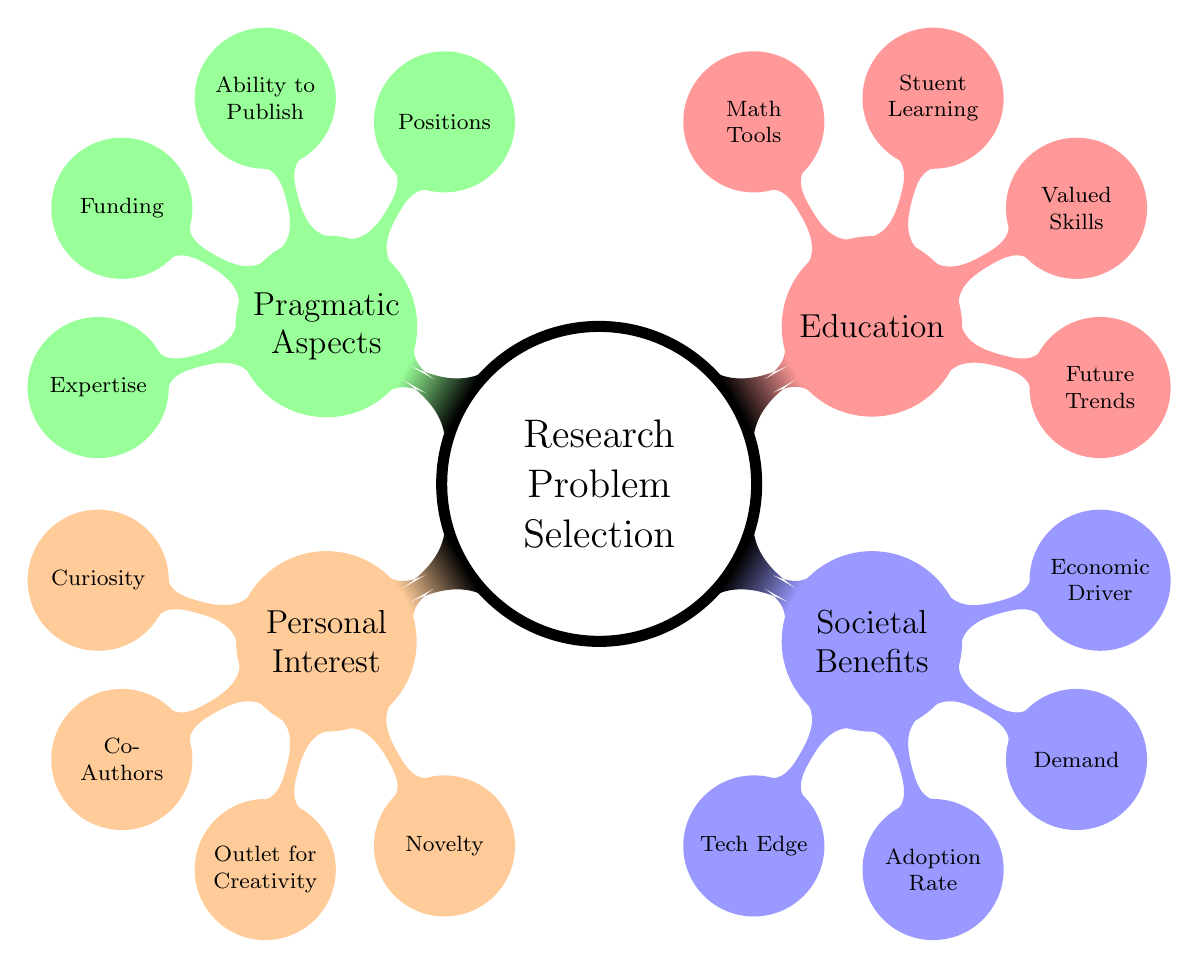
\begin{tikzpicture}[mindmap]
  \begin{scope}[
    every node/.style={concept},
    Root/.append style={
      concept color=black, fill=white, line width=4pt, font=\Large},
    Education/.style={concept color=red!40,grow=30},
    Society/.style={concept color=blue!40,grow=330},
    Interest/.style={concept color=orange!40,grow=210},
    Pragmatism/.style={concept color=green!40,grow=150},
    grow cyclic,
    level 1/.append style={level distance=4cm,font=\large},
    level 2/.append style={level distance=3cm,sibling angle=90}]
    \node [Root] {Research Problem Selection} %  root
      child [Education] { node {Education}
        child [grow=120] { node {Math Tools} }
        child [grow=75] { node {Stuent Learning} }
        child [grow=30] { node {Valued Skills} }
        child [grow=345] { node {Future Trends} }
      }
      child [Society] { node {Societal Benefits}
        child [grow=15] { node {Economic Driver} }
        child [grow=330] { node {Demand} }
        child [grow=285] { node {Adoption Rate} }
        child [grow=240] { node {Tech Edge} }
      }
      child [Interest] { node {Personal Interest}
        child [grow=165] { node {Curiosity} }
        child [grow=210] { node {Co-Authors} }
        child [grow=255] { node {Outlet for Creativity} }
        child [grow=300] { node {Novelty} }
      }
      child [Pragmatism] { node {Pragmatic Aspects}
        child [grow=60] { node {Positions} }
        child [grow=105] { node {Ability to Publish} }
        child [grow=150] { node {Funding} }
        child [grow=195] { node {Expertise} }
      };
  \end{scope}
\end{tikzpicture}
}
  \end{center}
\end{frame}

\begin{frame}
  \frametitle{Education: Seeking Long-Term Impact}

  \begin{center}
  \scalebox{0.5}{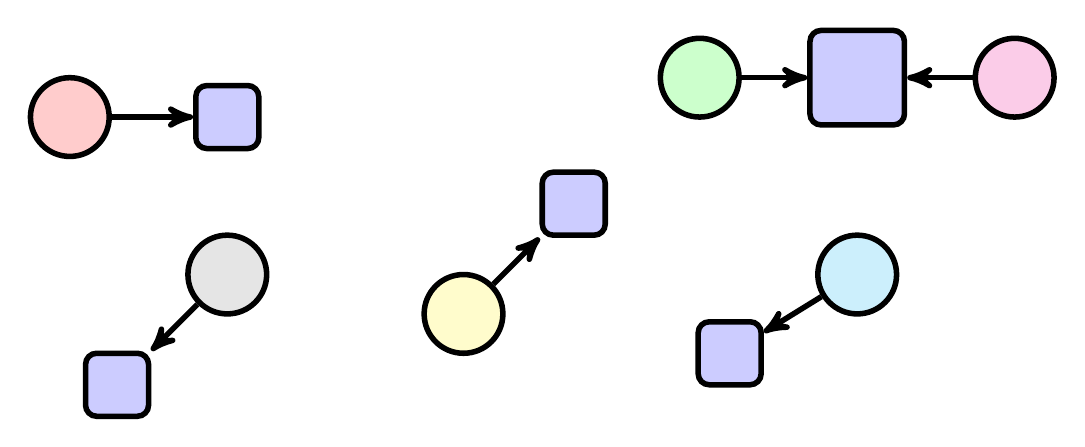
\begin{tikzpicture}
[draw=black, line width=2pt, >=stealth',
author/.style={circle, draw, inner sep=0pt, minimum size=10mm},
contribution/.style={rectangle, draw, inner sep=0pt, minimum size=8mm, fill=blue!20, rounded corners}]

\node[author, fill=red!20] (author1) at (0,2) {};
\node[contribution] (contribution1) at (2,2) {}
  edge [<-] (author1);
\node[author, fill=gray!20] (author2) at (2,0) {};
\node[contribution] (contribution2) at (0.6,-1.4) {}
  edge [<-] (author2);
\node[author, fill=green!20] (author3) at (8,2.5) {};
\node[author, fill=magenta!20] (author4) at (12,2.5) {};
\node[contribution, minimum size=12mm] (contribution3) at (10,2.5) {}
  edge [<-] (author3)
  edge [<-] (author4);
\node[author, fill=yellow!20] (author5) at (5,-0.5) {};
\node[contribution] (contribution5) at (6.4,0.9) {}
  edge [<-] (author5);
\node[author, fill=cyan!20] (author6) at (10,0) {};
\node[contribution] (contribution6) at (8.38,-1) {}
  edge [<-] (author6);
\end{tikzpicture}

} \\
  \emph{Isolated efforts result in duplicated tasks}
  \end{center}
  \begin{block}{Collective Opportunities}
    \begin{enumerate}
    \item Devoting time to building lasting tools enhances productivity of instructors and elevate quality of programs over time
    \item Working jointly in cohesive framework leads to great achievements whose values far exceed individual contributions
    \end{enumerate}
  \end{block}
\end{frame}

\begin{frame}
  \frametitle{Education: Lessons from Software Development}

  \begin{center}
  \scalebox{0.5}{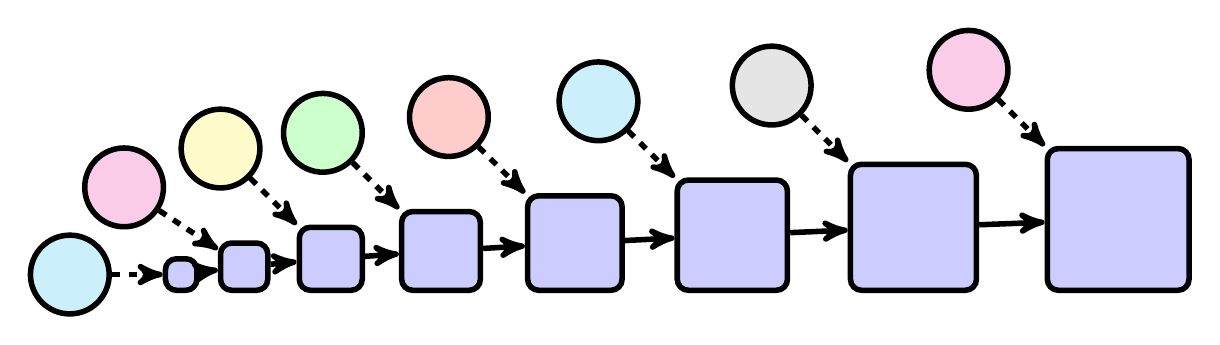
\begin{tikzpicture}
[draw=black, line width=2pt, >=stealth',
author/.style={circle, draw, inner sep=0pt, minimum size=10mm},
contribution/.style={rectangle, draw, inner sep=0pt, minimum size=18mm, fill=blue!20, rounded corners}]

\node[contribution, minimum size=4mm] (project1) at (0,0.2) {};
\node[contribution, minimum size=6mm] (project2) at (0.8,0.3) {}
  edge [<-] (project1);
\node[contribution, minimum size=8mm] (project3) at (1.9,0.4) {}
  edge [<-] (project2);
\node[contribution, minimum size=10mm] (project4) at (3.3,0.5) {}
  edge [<-] (project3);
\node[contribution, minimum size=12mm] (project5) at (5,0.6) {}
  edge [<-] (project4);
\node[contribution, minimum size=14mm] (project6) at (7,0.7) {}
  edge [<-] (project5);
\node[contribution, minimum size=16mm] (project7) at (9.3,0.8) {}
  edge [<-] (project6);
\node[contribution, minimum size=18mm] (project8) at (11.9,0.9) {}
  edge [<-] (project7);
\node[author, fill=cyan!20] (author1) at (-1.4142,0.2) {}
  edge [->, dashed] (project1);
\node[author, fill=magenta!20] (author2) at (-0.7247,1.3071) {}
  edge [->, dashed] (project2);
\node[author, fill=yellow!20] (author3) at (0.5,1.8) {}
  edge [->, dashed] (project3);
\node[author, fill=green!20] (author5) at (1.8,2.0) {}
  edge [->, dashed] (project4);
\node[author, fill=red!20] (author5) at (3.4,2.2) {}
  edge [->, dashed] (project5);
\node[author, fill=cyan!20] (author6) at (5.3,2.4) {}
  edge [->, dashed] (project6);
\node[author, fill=gray!20] (author7) at (7.5,2.6) {}
  edge [->, dashed] (project7);
\node[author, fill=magenta!20] (author8) at (10,2.8) {}
  edge [->, dashed] (project8);
\end{tikzpicture}

} \\
  \emph{Pushing resources forward with version control}
  \end{center}
  \begin{block}{A Source of Inspiration}
    \begin{enumerate}
    \item Best practices can be inferred from software engineering and large open projects, e.g., GNU/Linux, FreeBSD, Apache, Mozilla/Firefox
    \item Software versioning and revision control systems can manage changes to educational documents and source files, e.g., \texttt{GitHub.com}
    \end{enumerate}
  \end{block}
\end{frame}

\begin{frame}
  \frametitle{Education: Shedding Light on the Snowball Effect}

  \begin{block}{Positive Points}
    \begin{enumerate}
    \item \emph{EduDocs:} Several instructor employ framework to create and maintain documents
    \item Hundreds of students have used notes
    \item Licensing facilitates content reuse
    \end{enumerate}
  \end{block}
  \vfill
  \begin{block}{Drawbacks}
    \begin{enumerate}
    \item Lack of \emph{synchronizing agent}
    \item Barriers to entry appear high
    %\item Several competing initiatives
    \end{enumerate}
  \end{block}
\end{frame}

\begin{frame}
  \frametitle{Education: Project-Based Courses}

  \begin{center}
  \scalebox{0.5}{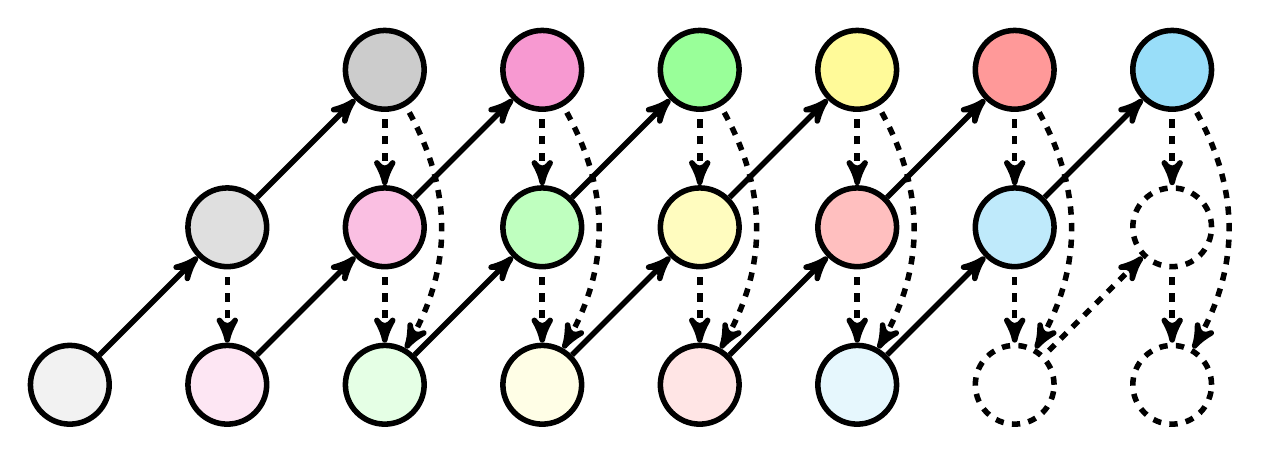
\begin{tikzpicture}
[draw=black, line width=2pt, >=stealth',
author/.style={circle, draw, inner sep=0pt, minimum size=10mm},
contribution/.style={rectangle, draw, inner sep=0pt, minimum size=18mm, fill=blue!20, rounded corners}]

\node[author, fill=gray!10] (author10) at (0,-2) {};
\node[author, fill=gray!25] (author11) at (2,0) {}
  edge [<-] (author10);
\node[author, fill=gray!40] (author12) at (4,2) {}
  edge [<-] (author11);
\node[author, fill=magenta!10] (author20) at (2,-2) {}
  edge [<-, dashed] (author11);
\node[author, fill=magenta!25] (author21) at (4,0) {}
  edge [<-, dashed] (author12)
  edge [<-] (author20);
\node[author, fill=magenta!40] (author22) at (6,2) {}
  edge [<-] (author21);
\node[author, fill=green!10] (author30) at (4,-2) {}
  edge [<-, dashed, bend right=30] (author12)
  edge [<-, dashed] (author21);
\node[author, fill=green!25] (author31) at (6,0) {}
  edge [<-, dashed] (author22)
  edge [<-] (author30);
\node[author, fill=green!40] (author32) at (8,2) {}
  edge [<-] (author31);
\node[author, fill=yellow!10] (author40) at (6,-2) {}
  edge [<-, dashed, bend right=30] (author22)
  edge [<-, dashed] (author31);
\node[author, fill=yellow!25] (author41) at (8,0) {}
  edge [<-, dashed] (author32)
  edge [<-] (author40);
\node[author, fill=yellow!40] (author42) at (10,2) {}
  edge [<-] (author41);
\node[author, fill=red!10] (author50) at (8,-2) {}
  edge [<-, dashed, bend right=30] (author32)
  edge [<-, dashed] (author41);
\node[author, fill=red!25] (author51) at (10,0) {}
  edge [<-, dashed] (author42)
  edge [<-] (author50);
\node[author, fill=red!40] (author52) at (12,2) {}
  edge [<-] (author51);
\node[author, fill=cyan!10] (author60) at (10,-2) {}
  edge [<-, dashed, bend right=30] (author42)
  edge [<-, dashed] (author51);
\node[author, fill=cyan!25] (author61) at (12,0) {}
  edge [<-, dashed] (author52)
  edge [<-] (author60);
\node[author, fill=cyan!40] (author62) at (14,2) {}
  edge [<-] (author61);
\node[author, dashed] (author70) at (12,-2) {}
  edge [<-, dashed, bend right=30] (author52)
  edge [<-, dashed] (author61);
\node[author, dashed] (author71) at (14,0) {}
  edge [<-, dashed] (author62)
  edge [<-, dashed] (author70);
\node[author, dashed] (author80) at (14,-2) {}
  edge [<-, dashed, bend right=30] (author62)
  edge [<-, dashed] (author71);
\end{tikzpicture}

} \\
  \emph{Foster cultures where students help students}
  \end{center}
  \begin{block}{Transferable Skills}
    \begin{enumerate}
    \item Engineering students must develop several facets: teamwork, programming and marketing skills, time management, creativity
    \item Project-based learning complements traditional classroom and assists students acquire these skills
    \end{enumerate}
  \end{block}
\end{frame}

\begin{frame}
  \frametitle{Education: Align Deliverables and Valuables}

  \begin{center}
  \scalebox{0.5}{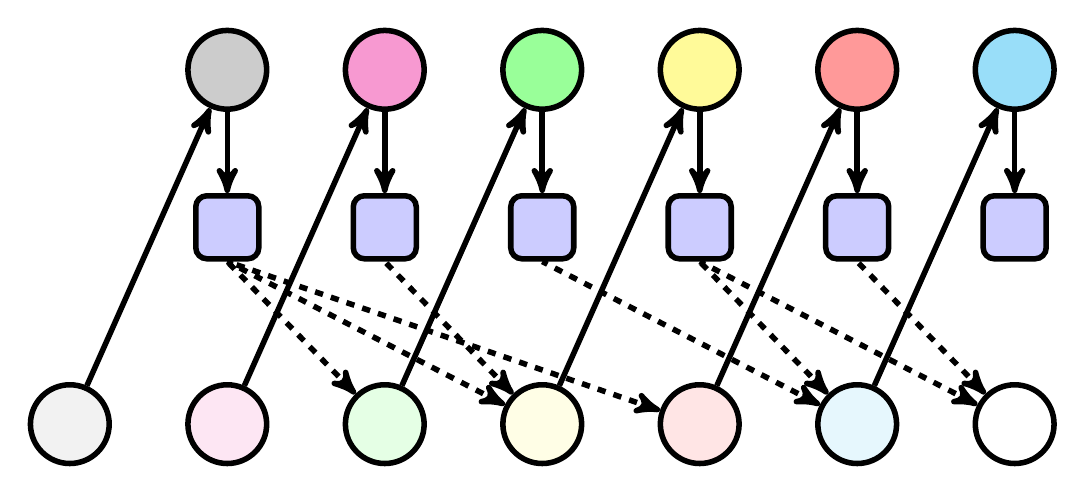
\begin{tikzpicture}
[draw=black, line width=2pt, >=stealth',
author/.style={circle, draw, inner sep=0pt, minimum size=10mm},
contribution/.style={rectangle, draw, inner sep=0pt, minimum size=8mm, fill=blue!20, rounded corners}]

\node[author, fill=gray!40] (author12) at (0,2.5) {};
\node[contribution] (project1) at (0,0.5) {}
  edge [<-] (author12);
\node[author, fill=magenta!40] (author22) at (2,2.5) {};
\node[contribution] (project2) at (2,0.5) {}
  edge [<-] (author22);
\node[author, fill=green!40] (author32) at (4,2.5) {};
\node[contribution] (project3) at (4,0.5) {}
  edge [<-] (author32);
\node[author, fill=yellow!40] (author42) at (6,2.5) {};
\node[contribution] (project4) at (6,0.5) {}
  edge [<-] (author42);
\node[author, fill=red!40] (author52) at (8,2.5) {};
\node[contribution] (project5) at (8,0.5) {}
  edge [<-] (author52);
\node[author, fill=cyan!40] (author62) at (10,2.5) {};
\node[contribution] (project6) at (10,0.5) {}
  edge [<-] (author62);

\node[author, fill=gray!10] (author10) at (-2,-2) {}
  edge [->] (author12);
\node[author, fill=magenta!10] (author20) at (0,-2) {}
  edge [->] (author22);
\node[author, fill=green!10] (author30) at (2,-2) {}
  edge [->] (author32);
  \path (author30) edge[<-, dashed] (project1.south);
\node[author, fill=yellow!10] (author40) at (4,-2) {}
  edge [->] (author42);
  \path (author40) edge[<-, dashed] (project2.south);
  \path (author40) edge[<-, dashed] (project1.south);
\node[author, fill=red!10] (author50) at (6,-2) {}
  edge [->] (author52);
  \path (author50) edge[<-, dashed] (project1.south);
\node[author, fill=cyan!10] (author60) at (8,-2) {}
  edge [->] (author62);
  \path (author60) edge[<-, dashed] (project3.south);
  \path (author60) edge[<-, dashed] (project4.south);
\node[author] (author70) at (10,-2) {};
  \path (author70) edge[<-, dashed] (project4.south);
  \path (author70) edge[<-, dashed] (project5.south);
\end{tikzpicture}

} \\
  \emph{Trust students to produce useful documents}
  \end{center}
  \begin{block}{Transferable Skills}
    \begin{enumerate}
    \item Reports get low readership, whereas tutorials can have broader appeal and can be leveraged to bootstrap future projects
    \item Setting goals that fulfill curriculum requirements and yield valuable outcomes can elevate quality of programs
    \end{enumerate}
  \end{block}
\end{frame}

\end{document}

